\documentclass[border=6pt]{standalone}
\usepackage{fontspec,unicode-math}
\setmainfont{Noto Serif}
\setmathfont{STIXTwoMath-Regular.otf}
\usepackage{tikz}
\usetikzlibrary{arrows.meta,calc,patterns,decorations.markings,decorations.pathmorphing,decorations.pathreplacing}
\tikzset{lev/.style={line width=1.18pt,line cap=butt},
 fine/.style={line width=.55pt},light/.style={line width=.4pt},
 curve/.style={line width=1.18pt,line cap=round,line join=round},
 ax/.style={line width=.62pt,-{Latex[length=2.15mm,width=1.2mm]}},
 ray/.style={line width=.64pt,-{Latex[length=1.9mm,width=1.0mm]}},
 dim/.style={line width=.52pt,{Latex[length=1.65mm,width=.85mm]}-{Latex[length=1.65mm,width=.85mm]}},
 flow/.style={line width=.60pt,postaction={decorate},decoration={markings,mark=at position .62 with {\arrow{Latex[length=1.9mm,width=1.0mm]}}}},
 lab/.style={font=\fontsize{13}{16}\selectfont,inner sep=1.5pt},
 small/.style={font=\fontsize{11.2}{13.5}\selectfont,inner sep=1.2pt},
 panel/.style={font=\fontsize{13}{16}\selectfont\itshape,inner sep=1.5pt}}
\pagestyle{empty}
\begin{document}
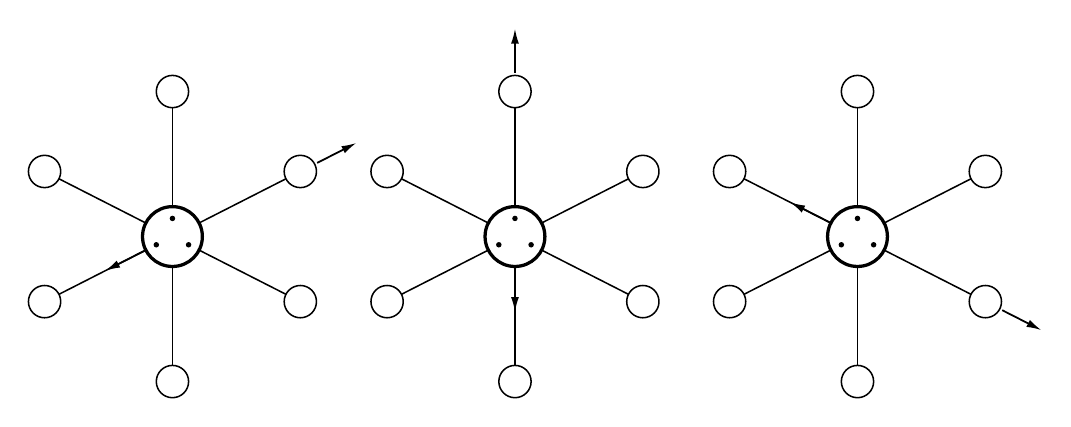
\begin{tikzpicture}[x=1cm,y=1cm,line join=round]
\draw[fine] (0.000000,0.000000)--(-1.624000,-0.826500);
\path[draw,fine,fill=white] (-1.624000,-0.826500) circle (.205);
\draw[fine] (0.000000,0.000000)--(1.624000,0.826500);
\path[draw,fine,fill=white] (1.624000,0.826500) circle (.205);
\draw[fine] (0.000000,0.000000)--(1.624000,-0.826500);
\path[draw,fine,fill=white] (1.624000,-0.826500) circle (.205);
\draw[fine] (0.000000,0.000000)--(-1.624000,0.826500);
\path[draw,fine,fill=white] (-1.624000,0.826500) circle (.205);
\draw[fine] (0.000000,0.000000)--(0.000000,-1.841500);
\path[draw,fine,fill=white] (0.000000,-1.841500) circle (.205);
\draw[fine] (0.000000,0.000000)--(0.000000,1.841500);
\path[draw,fine,fill=white] (0.000000,1.841500) circle (.205);
\path[draw,curve,fill=white] (0.000000,0.000000) circle (.38);
\fill (-0.204981,-0.104321) circle (.035);
\fill (0.204981,-0.104321) circle (.035);
\fill (0.000000,0.230000) circle (.035);
\draw[ray] (-0.356489,-0.181427)--(-0.855573,-0.435425);
\draw[ray] (1.837893,0.935356)--(2.336977,1.189355);
\draw[fine] (4.350000,0.000000)--(2.726000,-0.826500);
\path[draw,fine,fill=white] (2.726000,-0.826500) circle (.205);
\draw[fine] (4.350000,0.000000)--(5.974000,0.826500);
\path[draw,fine,fill=white] (5.974000,0.826500) circle (.205);
\draw[fine] (4.350000,0.000000)--(5.974000,-0.826500);
\path[draw,fine,fill=white] (5.974000,-0.826500) circle (.205);
\draw[fine] (4.350000,0.000000)--(2.726000,0.826500);
\path[draw,fine,fill=white] (2.726000,0.826500) circle (.205);
\draw[fine] (4.350000,0.000000)--(4.350000,-1.841500);
\path[draw,fine,fill=white] (4.350000,-1.841500) circle (.205);
\draw[fine] (4.350000,0.000000)--(4.350000,1.841500);
\path[draw,fine,fill=white] (4.350000,1.841500) circle (.205);
\path[draw,curve,fill=white] (4.350000,0.000000) circle (.38);
\fill (4.145019,-0.104321) circle (.035);
\fill (4.554981,-0.104321) circle (.035);
\fill (4.350000,0.230000) circle (.035);
\draw[ray] (4.350000,-0.400000)--(4.350000,-0.960000);
\draw[ray] (4.350000,2.081500)--(4.350000,2.641500);
\draw[fine] (8.700000,0.000000)--(7.076000,-0.826500);
\path[draw,fine,fill=white] (7.076000,-0.826500) circle (.205);
\draw[fine] (8.700000,0.000000)--(10.324000,0.826500);
\path[draw,fine,fill=white] (10.324000,0.826500) circle (.205);
\draw[fine] (8.700000,0.000000)--(10.324000,-0.826500);
\path[draw,fine,fill=white] (10.324000,-0.826500) circle (.205);
\draw[fine] (8.700000,0.000000)--(7.076000,0.826500);
\path[draw,fine,fill=white] (7.076000,0.826500) circle (.205);
\draw[fine] (8.700000,0.000000)--(8.700000,-1.841500);
\path[draw,fine,fill=white] (8.700000,-1.841500) circle (.205);
\draw[fine] (8.700000,0.000000)--(8.700000,1.841500);
\path[draw,fine,fill=white] (8.700000,1.841500) circle (.205);
\path[draw,curve,fill=white] (8.700000,0.000000) circle (.38);
\fill (8.495019,-0.104321) circle (.035);
\fill (8.904981,-0.104321) circle (.035);
\fill (8.700000,0.230000) circle (.035);
\draw[ray] (8.343511,0.181427)--(7.844427,0.435425);
\draw[ray] (10.537893,-0.935356)--(11.036977,-1.189355);

\end{tikzpicture}
\end{document}
